\documentclass[12pt]{article}}
\usepackage{fontspec}   %加這個就可以設定字體
\usepackage{xeCJK}       %讓中英文字體分開設置
\setmainfont{Times New Roman}
\setCJKmainfont{標楷體} %設定中文為系統上的字\cite{}型,而英文不去更動,使用原TeX字型
\XeTeXlinebreaklocale "zh"             %這兩行一定要加,中文才能自動換行
\XeTeXlinebreakskip = 0pt plus 1pt     %這兩行一定要加,中文才能自動換行
\usepackage{amsmath, amsthm, amssymb} %引入數學符號的套件,例如實數R、定理Thm...
\usepackage{graphicx}                 %現在, 假設我們要插入 pic.png 這個圖檔, 使用
%\title{我是標題}
%\author{我是作者}
%\date{} %不要日期

\newcommand{\uA}       {\mbox{\boldmath$A$}}
\usepackage{textcomp}
\usepackage{array}
\usepackage{graphicx}
\usepackage{colortbl}
\usepackage{color,xcolor}
\usepackage{listings}
\usepackage{array,booktabs}   %這三個為表格使用的套件
\usepackage{textpos}
\usepackage{float}
\usepackage{listings}

\title{Statistical learning assignment 9- chapter 5}
\author{孫浩哲 \hspace{0.7cm} M072040002}
\date{November 15, 2018}
\begin{document}
\maketitle
\begin{itemize}
\item[1.]
\begin{align*}
f(\alpha)
&=Var(\alpha X+(1-\alpha)Y)\\
&=\alpha^2Var(X)+(1-\alpha)^2Var(Y)+2\alpha(1-\alpha)Cov(X,Y)
\end{align*}
\begin{align*}
f'(\alpha)
&=2\alpha Var(X)-2(1-\alpha)Var(Y)+(2-4\alpha)Cov(X,Y)\\
&=[Var(X)+Var(Y)-2Cov(X,Y)]\alpha-Var(Y)+Cov(X,Y)=0\\[3ex]
&\Rightarrow\hat{\alpha}=\frac{Var(Y)-Cov(X,Y)}{Var(X-Y)}
\end{align*}
\item[2.]
(a)
The first bootstrap observation is the \ $jth$ observation from the original sample is $\frac{1}{n}$,
so the probability of opposite situation is\ $1-\frac{1}{n}$.\\[2ex]
(b)
Same as (a), $1-\frac{1}{n}$\\[2ex]
(c)
The probability that we don't get \ $jth$ observation in single sampling is $1-\frac{1}{n}$,so the probability that the\ $jth$ observation is not in the bootstrap sample is \ $(1-\frac{1}{n})^n$\\[2ex]
(d)
$1-(1-\frac{1}{5})^5=\frac{2101}{3125}\approx67.2\%$\\[2ex]
(e)
$1-(1-\frac{1}{100})^{100}\approx63.4\%$\\[2ex]
(f)
$1-(1-\frac{1}{10000})^{10000}\approx1-e^{-1}\approx63.2\%$
\newpage
(g)\\
\raggedright{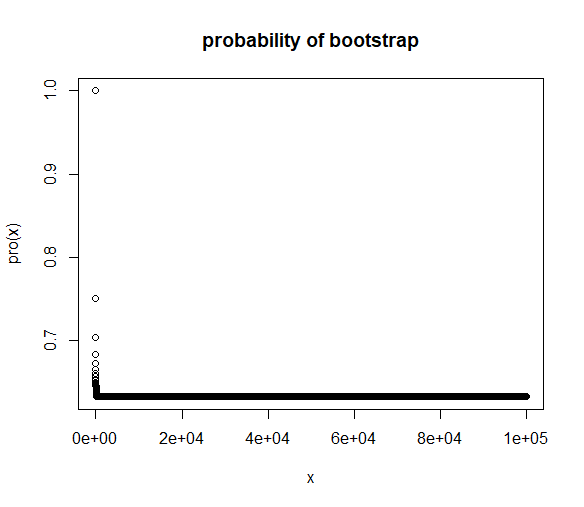
\includegraphics[width=0.8\linewidth]{bootstrap}}\\[2ex]
The probability converges to \ $0.632$.\\[2ex]
(f)\\
Denoted the probability that a bootstrap sample of size\ $n=100$ not contains the\ $4th$ observation as\ $p$.\\[2ex]
As we repeated sampling, the\ $p$ is close to\ $0.634$.
\item[3.]
(a)\ \\
We take the set of n observations, and divide into\ $k$ groups which are non-overlapping, and we choose one group as validation group and the other\ $k-1$ groups as training set each time.We estimate the test error by averaging mean square error we get each time.\\[3ex]
(b)\ \\
\ (i) advantages:simple\\
\ \ \ \ \ disadvantages:estimate of test error rate can be highly variable.\\
\ (ii)advantages:small bias\\
\ \ \ \ \ disadvantages:high variance that attribute to many folds.
\item[8.]
(a)\ \\
\ $n=100,p=2$\ \ \ \ $Y=X-2X^2+\epsilon$, $\epsilon\sim N(0,1)$\\[2ex]
(b)\\
\raggedright{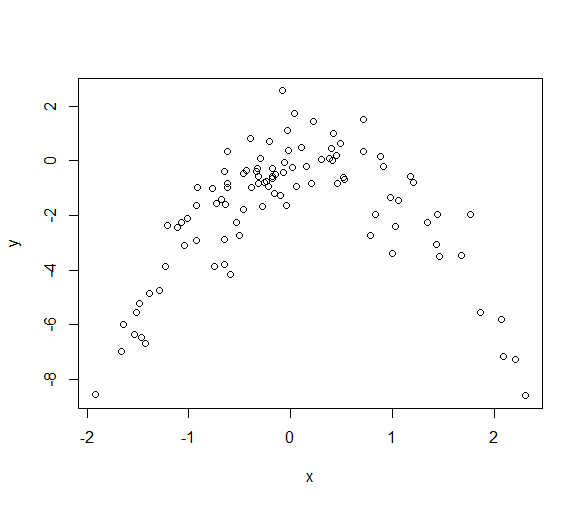
\includegraphics[width=0.8\linewidth]{square}}\\
(c)
\begin{verbatim}
> model=glm(y~x)
> cv.glm(data,model)$delta
[1] 5.890979 5.888812
> model2=glm(y~x+I(x^2))
> cv.glm(data,model2)$delta
[1] 1.086596 1.086326
> model3=glm(y~x+I(x^2)+I(x^3))
> cv.glm(data,model3)$delta
[1] 1.102585 1.102227
> model4=glm(y~x+I(x^2)+I(x^3)+I(x^4))
> cv.glm(data,model4)$delta
[1] 1.114772 1.114334
\end{verbatim}
(d)
\begin{verbatim}
> {
+ set.seed(100)
+ y = rnorm(100)
+ x = rnorm(100)
+ y = x - 2 * x^2 + rnorm(100)
+ }
> data=data.frame(x,y)
> model=glm(y~x)
> cv.glm(data,model)$delta
[1] 5.780657 5.777577
> model2=glm(y~x+I(x^2))
> cv.glm(data,model2)$delta
[1] 1.096349 1.095750
> model3=glm(y~x+I(x^2)+I(x^3))
> cv.glm(data,model3)$delta
[1] 1.080556 1.079737
> model4=glm(y~x+I(x^2)+I(x^3)+I(x^4))
> cv.glm(data,model4)$delta
[1] 1.158939 1.157565
\end{verbatim}
slighty different, but the difference of delta of LOOCV is smaller than\ $k$-folds, it is because every single observation is one fold.\\[2ex]
(e)\ \\
The quadratic polynomial had the smallest LOOCV error when random seed =\ $1$, because we set that\ $Y=X-2X^2+\epsilon$\\[2ex]
(f)
\begin{verbatim}
> summary(model4)

Call:
glm(formula = y ~ x + I(x^2) + I(x^3) + I(x^4))

Deviance Residuals:
    Min       1Q   Median       3Q      Max
-2.7254  -0.6441   0.1544   0.6022   2.5396

Coefficients:
            Estimate Std. Error t value Pr(>|t|)
(Intercept)  0.06994    0.13587   0.515    0.608
x            1.06124    0.22321   4.754 7.07e-06 ***
I(x^2)      -2.03463    0.28653  -7.101 2.24e-10 ***
I(x^3)      -0.18382    0.08395  -2.190    0.031 *
I(x^4)      -0.01584    0.07365  -0.215    0.830
---
Signif. codes:  0 ‘***’ 0.001 ‘**’ 0.01 ‘*’ 0.05 ‘.’ 0.1 ‘ ’ 1

(Dispersion parameter for gaussian family taken to be 0.9886131)

    Null deviance: 529.969  on 99  degrees of freedom
Residual deviance:  93.918  on 95  degrees of freedom
AIC: 289.51

Number of Fisher Scoring iterations: 2
\end{verbatim}
Yes, because the degree of\ $1$ and degree of\ $2$ terms are really significant.
\item[9.]
(a)(b)
\begin{verbatim}
> mean(medv)
[1] 22.53281
> sd(medv)/sqrt(nrow(Boston))
[1] 0.4088611
\end{verbatim}
(c)
\begin{verbatim}
> boot(medv,bt,1000)

ORDINARY NONPARAMETRIC BOOTSTRAP


Call:
boot(data = medv, statistic = bt, R = 1000)


Bootstrap Statistics :
    original       bias    std. error
t1* 22.53281 -0.005832609   0.3992782
\end{verbatim}
It is little smaller than our answer from (b).
(d)
\begin{verbatim}
> t.test(medv)

	One Sample t-test

data:  medv
t = 55.111, df = 505, p-value < 2.2e-16
alternative hypothesis: true mean is not equal to 0
95 percent confidence interval:
 21.72953 23.33608
sample estimates:
mean of x
 22.53281
\end{verbatim}
$$[22.53281\pm2\times0.4]=[21.73281,22.33281]$$
The confidence interval we get from bootstrap is almost the same as we get in t.test.
(e)
\begin{verbatim}
> median(medv)
[1] 21.2
\end{verbatim}
(f)
\begin{verbatim}
> med=numeric(10000)
> for(i in 1:10000)
+ {
+   med[i]=median(sample(medv,250))
+ }
> sd(med)
[1] 0.3809128
\end{verbatim}
\begin{verbatim}
> me=function(data,i)
+ {
+ return(median(data[i]))
+ }
> boot(medv,me,1000)

ORDINARY NONPARAMETRIC BOOTSTRAP


Call:
boot(data = medv, statistic = me, R = 1000)


Bootstrap Statistics :
    original   bias    std. error
t1*     21.2 -0.01235   0.3630727
\end{verbatim}
The variance of bootstrap we get is smaller than the variance we estimate.
(g)
\begin{verbatim}
> quantile(medv,0.1)
  10%
12.75
\end{verbatim}
(h)
\begin{verbatim}
> qua=numeric(10000)
>
> for(j in 1:10000)
+ {
+   qua[j]=quantile(sample(medv,250),c(0.1))
+ }
> sd(qua)
[1] 0.497367
\end{verbatim}
\begin{verbatim}
> quan=function(data,i)
+ {
+ return(quantile(data[i],0.1))
+ }
> boot(medv,quan,1000)

ORDINARY NONPARAMETRIC BOOTSTRAP


Call:
boot(data = medv, statistic = quan, R = 1000)


Bootstrap Statistics :
    original   bias    std. error
t1*    12.75 -0.02455   0.4962873
\end{verbatim}
Both of them are almost the same.
\end{itemize}
\end{document} 